
\begin{document}

\maketitle

\section{Sissejuhatus}
\begin{frame}[fragile]
  \frametitle{Täna kavas}
\begin{itemize}
	\item Sissejuhatus
	\begin{itemize}
		\item Tutvumine
		\item Õppe struktuur
		\item Kodukord
		\item Aine struktuur
	\end{itemize}
	\item Äristrateegia ja IT seosed
	\item Arhitektuur
\end{itemize}
	
\end{frame}

\begin{frame}[fragile]
	\frametitle{Andres Kütt}
	\begin{columns}[t]
		\begin{column}{7cm}
			\begin{itemize}
				\item Raha eest programme tegemas aastast 1993
				\item Viimased kümmekond aastat arhitekt
				\item $\approx$MSc (UT, Statistika), MBA (EBS), MSc (MIT)
				\item Hetkel Riigi Infosüsteemi arhitekt
				\item Minevikus Skype, Hansapank, EMTA jne. + natuke konsultatsiooni
				\item Palju eri loenguid ja kursusi eri koolides
			\end{itemize}
		\end{column}
		\begin{column}[T]{3cm}
			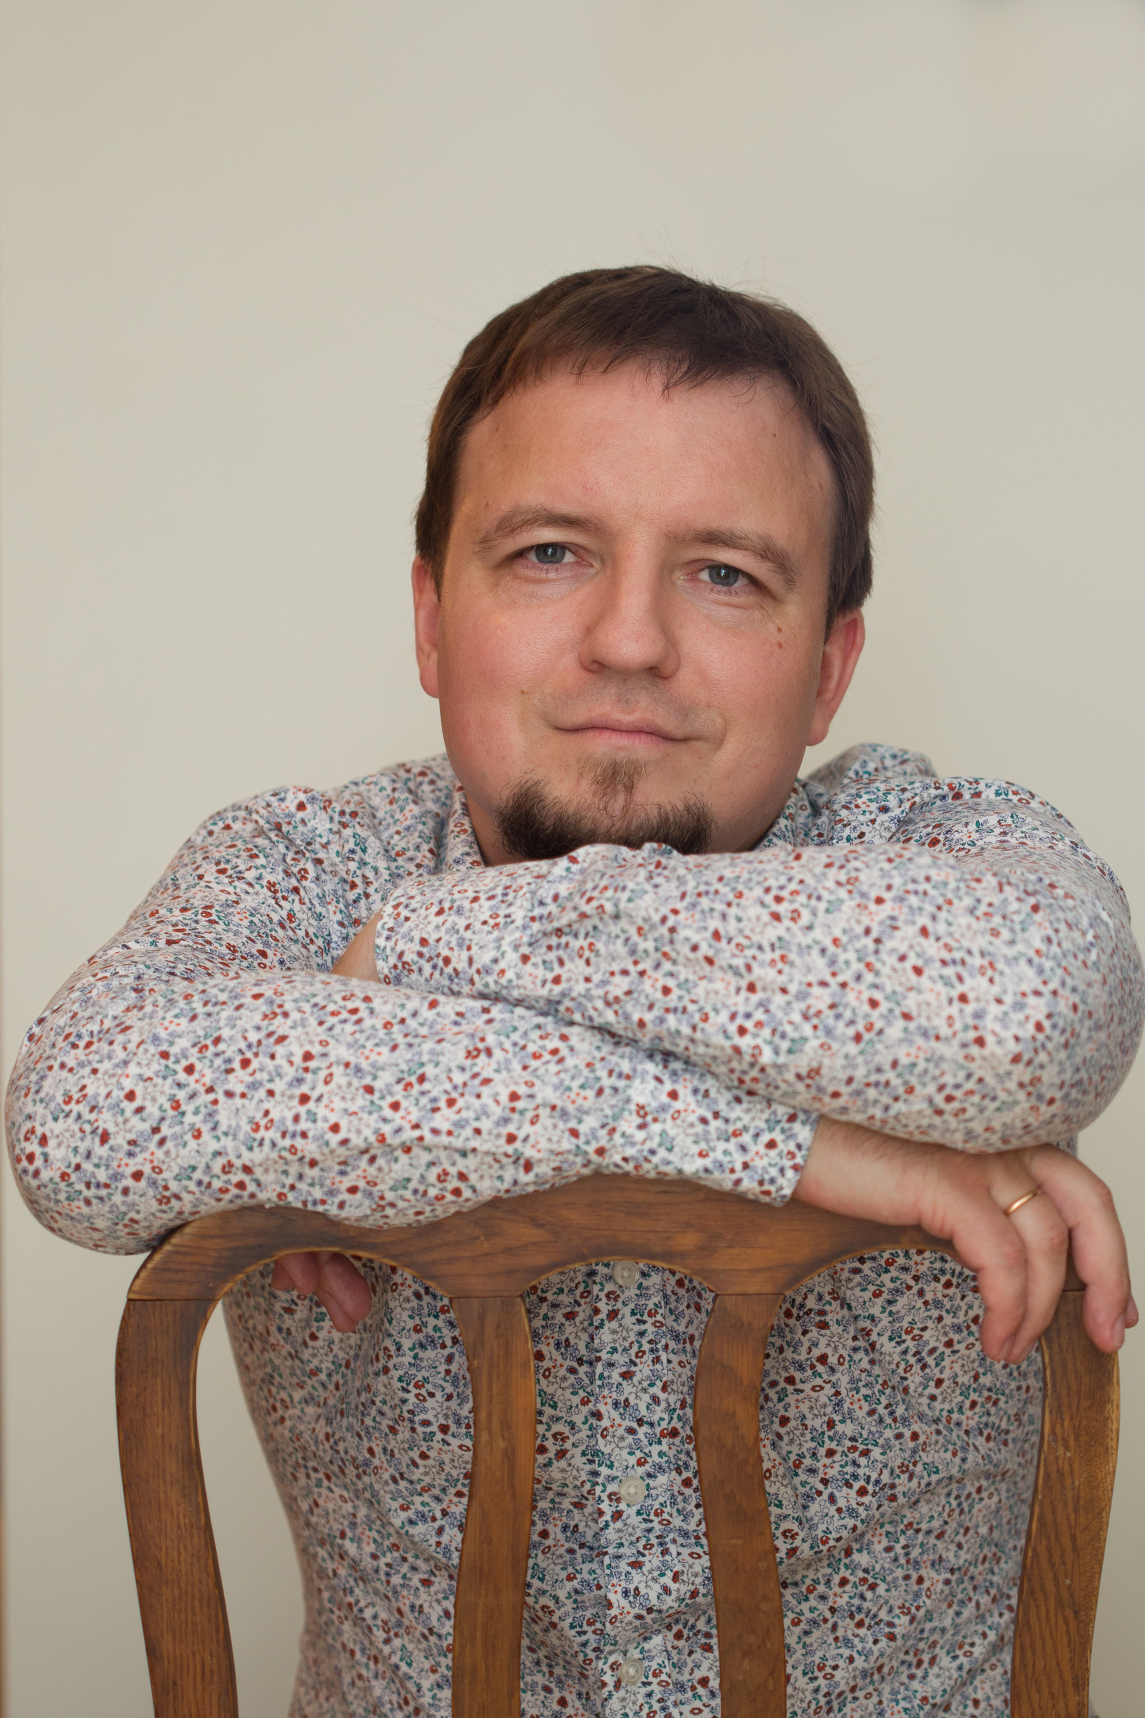
\includegraphics[width=\textwidth]{author.jpg}
		\end{column}
	\end{columns}
\end{frame}

\begin{frame}[fragile]
  \frametitle{Õppe struktuur}
	\begin{itemize}
	\item Loengud
	\begin{itemize}
		\item Igal kohtumisel 6 30-minutilist blokki
		\item Igas blokis 20 minutit juttu, 5 minutit arutelu paarides ja 5 minutit avalikku arutelu
		\item Loengus osalemine ei ole kohustuslik, seminaris osalemine on
	\end{itemize}
	\item \textbf{Rühmatöö:} IT strateegia koostamine ja esitamine rühmas
	\item \textbf{Eksam:} Kirjalik analüütiline töö

	\end{itemize}
\end{frame}

\begin{frame}[fragile]
  \frametitle{Rühmatööst}
Eesmärk on läbida IT strateegia koostamine \emph{võimalikult realistlikes} tingimustes 
  	\begin{itemize}
		\item Rühmatöö annab 70\% hindest
		\item Grupi suurus: $2\leq N\leq6$. \textbf{Ei mingeid erandeid!}
		\note{Hakake kohe gruppi otsima \par}
		\item Äri- ja IT strateegia vahelist piiri ette ei kirjutata
		\item Päädib suulise ettekandega, mille materialid esitatakse õppejõule ettekande järel kas dokumendi või esitlusena
		\item Edukriteerium: ettevõttel läheb dokumenti järgides usutavalt paremini, kui ilma selleta
		\item Hindamiskriteerium: ruumis esitatud küsimused saavad pädeva vastuse
	\end{itemize}
\end{frame}
\note{Kodutöö ja selle ette kandmine on kõige olulisem asi siin aines}

\begin{frame}[fragile]
  \frametitle{Kogemused kodutööst}
  	\begin{itemize}
		\item Ärge võtke liiga keerulisi ülesandeid
		\note{Eesmärgiks on markeerida strateegia tekitamise protsess, mitte välja mõelda lahendusi}
		\begin{itemize}
			\item Välja mõeldud organisatsioon on raskem, kui reaalne
			\item Riigiasutus on raskem, kui äriettevõte
			\item Väike organisatsioon on lihtam, kui suur
		\end{itemize}
		\item Mõistlik on tugineda aine struktuurile: kõik teemad võiksid ühel või teisel moel kaetud olla
		\item Tooge välja selge seos äristrateegiaga
		\begin{itemize}
			\item Ei ole mõistlik dikteerida ettevõtte strateegilisi valikuid
			\item On mõistlik ära tuua strateegilised piirangud
		\end{itemize}
		\item Pöörake tähelepanu esitlusele: kui te ei suuda infot edasi anda, ei ole seda olemas
	\end{itemize}
\end{frame}


\begin{frame}[fragile]
  \frametitle{Eksamist}
  Eksamiks on kahe või rohkema punktiga kirjalik analüütiline töö
  	\begin{itemize}	
		\item Küsimused on meie ühise arutelu küsimuste hulgast
		\item Hinnatakse sisu, mitte mahtu
		\item Kogemus võiks toimida: kui vastus on loengule tuginemata ammendav, on kõik hästi
		\note{Aga see on päris keeruline: teada tuleb ka diskussiooni käigus välja tulnut}
		\item Kui kodutöö on 100\%, eksamit vaja ei ole
		\item Eksam annab 30\% hindest
		\note{Kui olete hindega rahul, muidugi. Lugege ainekaarti!}
	\end{itemize}
\end{frame}

\begin{frame}[fragile]
  \frametitle{Õppe struktuur. Materjalid}
	\begin{itemize}
		\item Teen slaidid aga juttu läbi ei kirjuta
		\begin{itemize}
			\item Vähemalt ei saa seda lubada
			\item Kui keegi koostab mõistliku konspekti, aitan seda toimetada ja avaldada
			\item Tegelen kursuse raames tehnoloogilise loenguinnovatsiooniga \url{https://github.com/andreskytt/it_strateegia}!
		\end{itemize}
		\item Kõik vabalt saada olevad tekstid ja slaidid tekivad Moodlisse
		\item Kohustuslikku kirjandust ei ole sest teema on liiga lai ja inimeste võimalused erinevad
		\item Soovituslikku kirjandust viitan jooksvalt ja panen slaidide lõppu 
		\item Eraldi failis on erinevad märkused ning koondbibliograafia
	\end{itemize}
\note{Kogu asi on olemas githubis, sinna võib muutusi teha. Tegu on pedagoogilise eksperimendiga, eks näis, kuidas läheb. }
\end{frame}


\begin{frame}[fragile]
  \frametitle{Kodukord}
	\begin{itemize}
		\item Lubatud
		\begin{itemize}
			\item Küsimused ja õppejõu seisukohtade vaidlustamine
			\item Oma kogemuse mõõdukas jagamine
			\item Saabumine ja lahkumine millal iganes
		\end{itemize}
		\item Keelatud
		\begin{itemize}
			\item Aja raiskamine. Nii teie enese kui meie ühise aja.
		\end{itemize}
	\end{itemize}
\end{frame}
\note{On oluline vahe oma kogemuse jagamisel ja mõõdutul jauramisel, sama käib küsimuste kohta}

\begin{frame}[fragile]
  \frametitle{Aine struktuur}
	\begin{itemize}
		\item Tuginen IT Juhi kutsestandardile \citep{kutsestandard}
			\begin{itemize}
				\item Markeerin teemad, mida mujal kaetakse
				\item Tegelen jõudu mööda katmata teemadega
				\item Eesmärgiks anda tervikvaade
			\end{itemize}
		\item Tegelen põhimõtteliste asjadega
			\begin{itemize}
				\item Strateegia ülesandeks on vastata küsimusele “Kuidas me teeme asju paremini, kui teised” \citep{de2006strategy}	
				\item Seega on vaja aru saada aluspõhimõtetest
				\item Pealisehitus on nii ehk naa muutlik ja mitte-akadeemiline
			\end{itemize}
	\end{itemize}
\end{frame}
\note{ITILit, TOGAFi, COBITit, Scrumi jne. jne. jne. saate ise ka uurida. Nende mood muutub ja tegu ei ole akadeemilises mõttes relevantsete asjadega. Teadus on siiski teadus.}

\begin{frame}[fragile]
  \frametitle{Aine struktuur}
		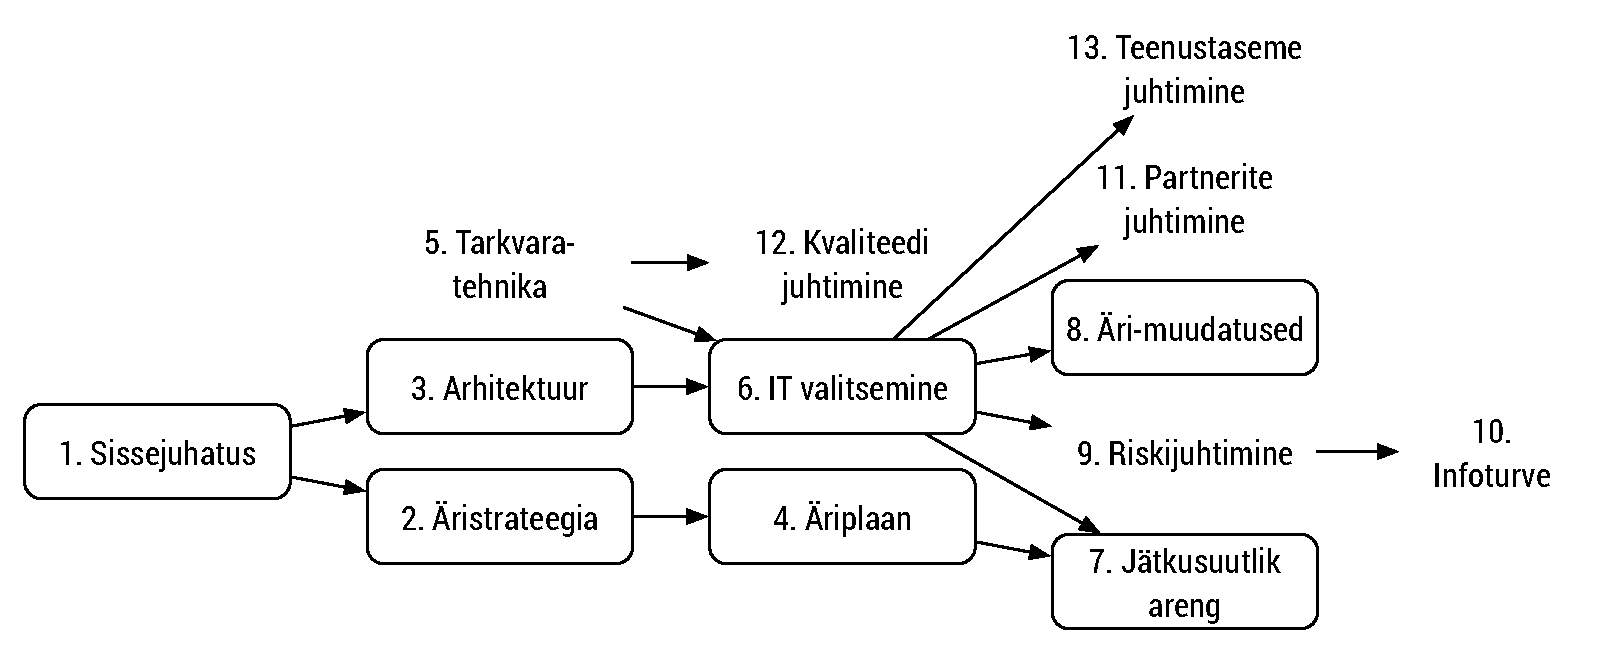
\includegraphics[width=\textwidth]{aine_struktuur.pdf}
\end{frame}
\note{Numbrid näitavad teemade esitamise järjekorda. Kastiga on sügavamalt käsitletavad teemad, ilma on asjad, mida mujal põhjalikult läbi räägitakse}

%Arutelu koht
\begin{frame}[fragile]
  \frametitle{Arutelu koht}
		\begin{center}
			\textbf{Mis on ootused sellele ainele?}
		\end{center}
\end{frame}
		
\section{Äristrateegia ja IT seosed}

\begin{frame}[fragile]
  \frametitle{Hommikusöögist}
  \begin{quote}
    Culture eats strategy for breakfast
  \end{quote}
	Peter Drucker
\end{frame}


\begin{frame}[fragile]
  \frametitle{Mis on strateegia?}
  	Võiks arvata, et strateegia mõiste on hästi määratletud. Siiski on paljul strateegiaks peetul strateegiaga vähe pistmist \citep{de2006strategy}. Dimensioonid on siiski paigas:
	\begin{itemize}
		\item Organisatsiooni postisioneerimine konkurentsieelise saamiseks
		\item Valik majandussektoris osalemise ning teenuste ja toodete pakkumise osas
		\item Ressursside suunamine 
	\end{itemize}
	\textbf{Eesmärk:} Väärtuse loomine omanikele ning teistele osapooltele läbi kliendile väärtuse pakkumise.
	\note{Mis on "väärtus" omaniku ja mis kliendi jaoks, on mittetriviaalne küsimus}
\end{frame}

\begin{frame}[fragile]
  \frametitle{Strateegia on dünaamiline}
	\vfill
	\begin{center}
		Strateegia peab muutuma vähemalt sama kiiresti, kui muutub omaniku ja kliendi arusaam väärtusest.
		\note{Tänapäeval tõenäoliselt kiiremini. Kolmandal kontaktil räägime sellest lähemalt.}
	\end{center}
	\vfill
\end{frame}


\begin{frame}[fragile]
  \frametitle{Sõjakunst}
  \emph{"Stratagos"} - Kreeka keeles väejuht. Sun Tzu "sõjakunst" \citep{tzu2013art} on siiani rakendatav:
  
  Võidul on viis osist. Võidab see, 
   \begin{enumerate}
   		\item kes teab, millal võidelda ja millal mitte
		\item kes teab, kuidas toimida tugevama ja nõrgema vastasega
		\item kelle armee kõik astmed on täidetud samast vaimust
		\item kes, olles ise valmis, ootab, tabamaks vastane ootamatult
		\item kellel on suveräänist segamata sõjaline võimekus
   \end{enumerate}
\end{frame}

\begin{frame}[fragile]
  \frametitle{Sõjakunst}
  \begin{quote}
    All warfare is based on deception
  \end{quote}

\end{frame}

\begin{frame}[fragile]
  \frametitle{Strateegia laiemas kontekstis}
  Strateegia on osa laiemast organisatsiooni juhtimise süsteemistkuhu kuuluvad veel kindlasti 
  	\begin{description}
		\item[Visioon] kui nägemus ühisest helgest tulevikust
		\item[Missioon] kui põhjus eksisteerida
		\item[Kultuur] kui komplekt kooseksisteerimist võimaldavaid väärtusi
	\end{description}	
	\begin{quote}
	vision = mission + strategy + culture \end{quote}\citep{lipton1996demystifying}
\end{frame}


\begin{frame}[fragile]
  \frametitle{Strateegia dünaamikast}
  On selge, et 
  \begin{itemize}
  	\item muutub keskkond
	\note{Globaliseerumise tõttu üha kiiremad ja raskemini ennustatavad\\}
	\item organisatsioon ise muutub
	\note{Me kõik inimestena vananeme või vahetume, see tingib muutusi\\}
	\item muutuvad kliendi ja omaniku arusaamad neile väärtuslikust
  \end{itemize}
  Seega on strateegia olemuselt dünaamiline nähtus. Järelikult
	\begin{itemize}
		\item Aegub ta varem või hiljem
		\item Tekitab liigne strateegiasse klammerdumine varem või hiljem lõhe juhtkonna ja töötajate vahele
		\note{Juhil on reaalsust palju lihtsam ignoreerida, kui sellega vahetult kokku puutuval töötajal}
	\end{itemize}
\end{frame}

\begin{frame}[fragile]
  \frametitle{Strateegia olemusest}
  Strateegiaga samaväärselt oluline on tema arendamise protsess. 
	\begin{itemize}
		\item Tulenevalt strateegia dünaamilisest olemusest, peab leiduma viis
		\begin{itemize}
			\item kuidas me muutusevajadusest teada saame ja sellele reageerime
			\item kuidas me strateegiat ignoreerime
			\note{Hädajuhtudeks on mõistlik omada hädaventiili, mis võimaldab strateegiast mööda minna\\}
			\item seda kõike teha ilma strateegia tõsiseltvõetavust kahjustamata
		\end{itemize}
		\item Ühise suuna määratlemine eeldab organisatsiooni võimet toime tulla eriarvamusega
		\item Ohule on kergem vastu astuda õlg õla kõrval. Strateegia arutelu annab kindluse, et ma lähme edasi kõik koos
		\note{Võib juhtuda, et julgusest on rohkem abi kui detailsest plaanist\\}
	\end{itemize}
\end{frame}

\begin{frame}[fragile]
  \frametitle{Strateegia kui jada otsuseid}
	Strateegiat võib vaadelda kui hulka otsuseid. Mida me teeme ja mida me \emph{ei tee}. Järelikult
	\begin{itemize}
		\item on strateegia loomisse, nagu igasse otsusesse, sisse ehitatud konflikt
		\note{Järelikult ei ole mõistlik hakata strateegiaga tegelema ilma võimekuseta konflikti juhtida\\}
		\item on strateegia aluseks edasistele otsustele (näiteks: projektide prioriteedid)
		\item ei tohi strateegiadokument olla "ümmargune"
	\end{itemize}
\end{frame}


%Arutelu koht
\begin{frame}[fragile]
  \frametitle{Arutelu koht}
		\begin{center}
			\textbf{Kuidas lahutada IT strateegia äristrateegiast?}
		\end{center}
\end{frame}

\begin{frame}[fragile,label={stack}]
	\frametitle{Organisatsiooni kihiline mudel}
	\begin{columns}[t]
		\begin{column}{6cm}
			\begin{itemize}
				\item Iga kiht on seotud eelmise ja järgmisega
				\item Illustreerib IT asukohta organisatsioonis arhitekti vaatepunktist
				\item Sarnane TOGAFi lähenemisele, kuid laiema tähendusega
			\end{itemize}
		\end{column}
		\begin{column}[T]{5cm}
			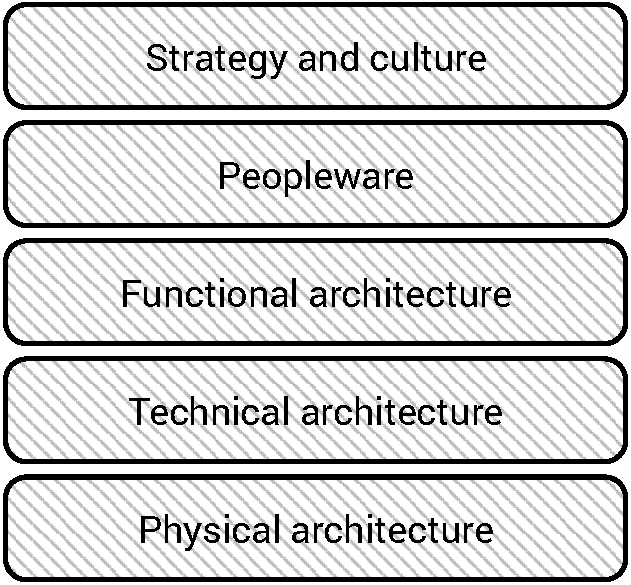
\includegraphics[width=\textwidth]{stack.pdf}
		\end{column}
	\end{columns}
\end{frame}

\begin{frame}[fragile]
  \frametitle{Kihid}
  	\begin{description}
		\item[Äri ja juriidika] Organisatsiooni strateegia ja juriidiline kontekst (seadusandlus, lepingud jne.)
		\item[Organisatsioon ja protsessid] Strateegiat realiseerivad org. struktuur ja äriprotsessid. Ka kultuur.
		\item[Funktsionaalsed komponendid] Protsesse toetavad funktsionaalsed komponendid (näiteks e-mail, ERP, veebipood, tootmisliin)
		\item[Tehnilised lahendused/IT] Funktsinaalsete komponentide tehniline/tehnoloogiline realisatsioon
		\item[Taristu] Tehniliste lahenduste taristu kuid ka näiteks kontorihooned
	\end{description}
\end{frame}

\begin{frame}[fragile]
  \frametitle{Järeldused mudelist}
	\begin{itemize}
		\item Kõik kihid on \emph{pidevas} muutumises, organisatsioon on dünaamiline nähtus
		\item Ükski muutus ei leia aset vaid ühes kihis
		\item Isoleeritud muutused tekitavad "tektoonilisi pingeid"
		\item Muutused propageeruvad üles ja alla tavaliselt kahaneva mõjuga
		\item IT ja äri kihid tavaliselt \emph{ainsad} üheselt juhitavad
	\end{itemize}
\end{frame}

%Arutelu koht
\begin{frame}[fragile]
  \frametitle{Arutelu koht}
		\begin{center}
			\textbf{Kui kiiresti muutused sumbuvad? Kas äristrateegia muutus võib muuta majutus-strateegiat?}
		\end{center}
\end{frame}

\begin{frame}[fragile]
  \frametitle{IT ja äri joondamine}
  IT eri aspektid ja organisatsioon toimivad pidevas dünaamilises tasakaalus. Vt. \cite{luftman2004assessing}
	\begin{columns}[t]
		\begin{column}{6cm}
			\begin{itemize}
				\item Osapooltel on vastandlikud huvid
				\item Oluline on huvide tasakaal
				\item Tasakaal tekib läbi organisatsiooni struktuuri ja protsesside
			\end{itemize}
		\end{column}
		\begin{column}[T]{5cm}
			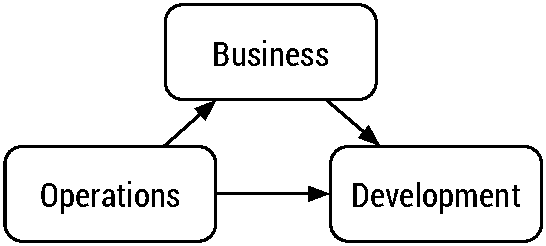
\includegraphics[width=\textwidth]{alignment.pdf}
		\end{column}
	\end{columns}
\end{frame}

\begin{frame}[fragile]
  \frametitle{IT kui integraalne osa organisatsioonist}
  Infotehnoloogiata ei ole mõeldavad terve rida organisatsiooni protsesse, ITl on nende kaudu oluline mõju äri toimivusele.
  \note{Ülidselt on raske ette kujutada organisatsiooni ilma ITta\\}
	\begin{itemize}
		\item ERP\footnote{Enterprise Resource Planning}
		\item Info/teadmus juhtimine
		\item Äriprotsesside juhtimine
	\end{itemize}
\end{frame}

\begin{frame}[fragile]
  \frametitle{IT mõju läbi {ERPi}}
  ERPi abil käivad ettevõtte paljud võtmeprotsessid: finants- ja personalijuhtimine, laohaldus jne. 
	\begin{itemize}
		\item ERPi suhteliselt väike probleem omab laialdast mõju
		\item Ettevõtte paindlikkus sõltub tema võimest muutusi ERPis kajastada
	\end{itemize}
  IT mõju näited:
	\begin{itemize}
		\item Milline partner või partnerid valitakse tarkvara pakkuma? 
		\item Kas ehitatame ise või ostame?
		\item Kuidas lahendatakse kasutajatoe ja majutuse küsimused? 
	\end{itemize}

\end{frame}

\begin{frame}[fragile]
  \frametitle{IT mõju läbi teadmusjuhtimise}
  Teadmus on ettevõtte jaoks kriitiline konkurentsieelis \citep{david2000diagnosing}. Tema juhtimine ilma tehnoloogiata ei ole lahenduv ülesanne. 
  	\begin{itemize}
		\item Loe teadmusjuhtimisest ja selle tehnilistest aspektidest \citep{15.905}
		\item Peamine järeldus: me ei saa teadmusjuhtimisest aru ja tegemist on kriitilise funktsiooniga. Seega tuleb talle läheneda väga ettevaatlikult.
	\end{itemize}
\end{frame}

\begin{frame}[fragile]
  \frametitle{IT mõju läbi äriprotsesside juhtimise}
		\begin{center}
			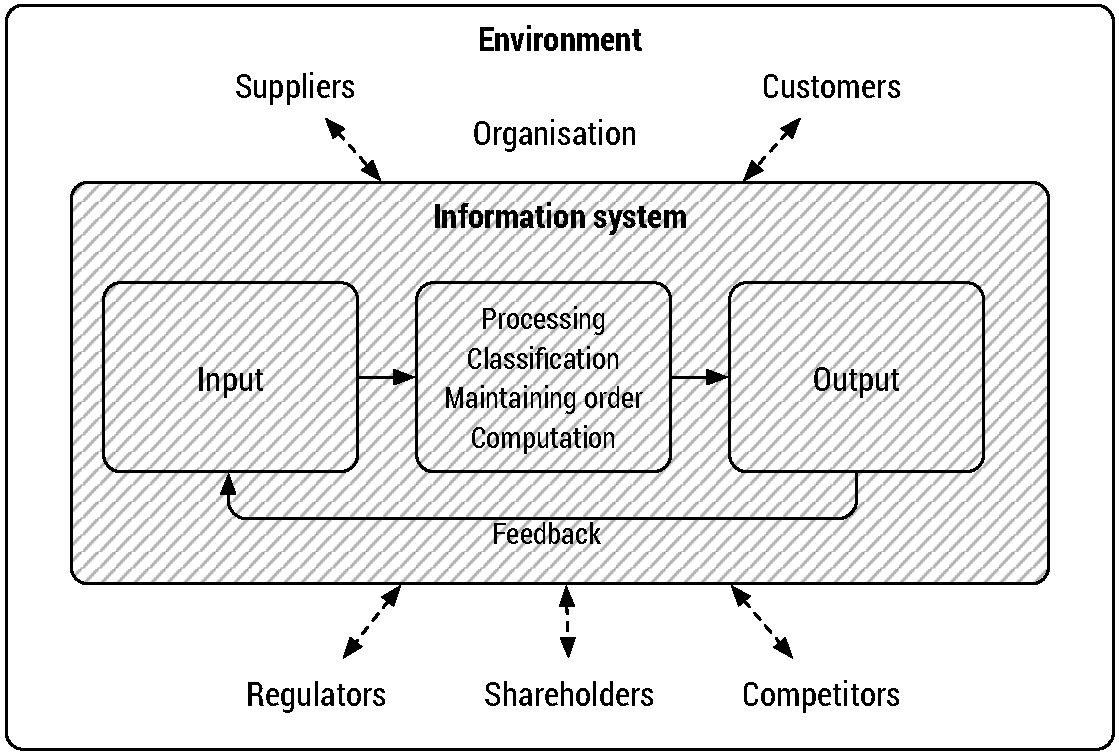
\includegraphics[width=.80\textwidth]{info_org.pdf}\\
		\end{center}
		\cite{laudon2000management}
\end{frame}


%Arutelu koht
\begin{frame}[fragile]
  \frametitle{Arutelu koht}
		\begin{center}
			\textbf{Kuidas juhtida mõistlikult IT kui organisatsioon kui tervik ei ole mõistlikult juhitud?}
		\end{center}
\end{frame}

\section{Arhitektuur}

\begin{frame}[fragile]
  \frametitle{Arhitektuuri tavapärane käsitlus}
		Inseneri vaates on arhitektuur kirjeldus sellest, kuidas millegi osad omavahel sobivad
		\begin{itemize}
			\item Toimiv ja end tõestanud praktika
			\item Hea arusaam tapi tugevusest ei anna vastust küsimusele, kuidas ehitada hea maja
		\end{itemize}
		
		Akadeemilises vaates on arhitektuur tavaliselt viis millegi formaalseks kirjeldamiseks ja selle kirjelduseni jõudmiseks
		\begin{itemize}
			\item Väga palju tööd millest väga vähe jõuab praktikasse
			\item Terve hulk omavahel sobimatuid paradigmasid
			\item Aitab mõelda vaid formaliseeritavatest asjadest
		\end{itemize}
		
\end{frame}

\begin{frame}[fragile]
	\frametitle{Vitruvius Pollio}
	\begin{columns}[t]
		\begin{column}{7cm}
			\begin{center}
				\begin{quote}
					\ldots all these must be built with due reference to durability, convenience and beauty
					\note{Vitruvian principles}
				\end{quote}
			\end{center}
			\vskip 1cm
			Marcus Vitruvius Pollio, 80-70 eKr.- 15 pKr  \citep{pollio1914vitruvius}
		\end{column}
		\begin{column}[T]{3cm}
			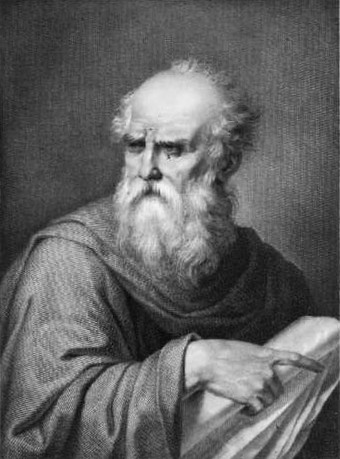
\includegraphics[width=\textwidth]{vitruvio.jpg}
		\end{column}
	\end{columns}
\end{frame}
\begin{frame}[label=Yosemite]
	\frametitle{Yosemite näide süsteemi piiridest}
	\begin{columns}[t]
		\begin{column}{6.5cm}
			Apple muutis 2014. teises pooles põhjalikult OS Xi kiipkaardi draiveriarhitektuuri
			\begin{itemize}
				\item Baastarkvaras muutust teha ei jõutud 
				\item 1. detsembril liitusid esimesed e-residendid
				\item Tulemuseks kallis ja närvesööv rabelemine
			\end{itemize}
		\end{column}
		\begin{column}[T]{4.5cm}
			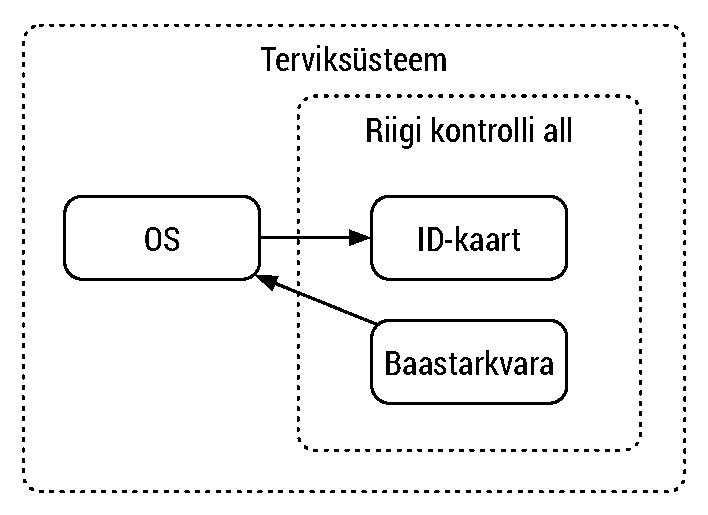
\includegraphics[width=\textwidth]{yosemite.pdf}
		\end{column}
	\end{columns}
\end{frame}


\begin{frame}[fragile]
  \frametitle{Süsteemi piiridest}
		Igasugune süsteemi piiri tõmbamine on meelevaldne
		\begin{itemize}
			\item Tavaliselt tehakse seda kas kontrolli või kompetentsi/tehnoloogia alusel
			\item Süsteemi võib kuuluda nii riistvara, tarkvara kui inimesed ning nendevahelised suhted
			\item Järelikult on meelevaldne rääkida vaid tarkvara või näiteks laua arhitektuurist
			\note{Eelnevalt ju rääkisime organisatsiooni arhitektuurist}
		\end{itemize}

\end{frame}

\begin{frame}
	\frametitle{Üldisemalt paradigmamuutusest}
	
	Järgmised tavapärased eeldused organisatsioonide kohta kehtivad üha harvemini
	\begin{enumerate}
		
	  	\item Organisatsioonid on kultuuriliselt, tehniliselt jne. homogeensed
		\note{Sina ja sinu arhitekuur võite pipramaale minna, ma tean paremini, mis töötab (kodanik Montevideost)\\}

		\item Organisatsioonilised ja juriidilised piirid on selgelt määratletud
		\note{Tihedalt integreeritud tarneahelad, Laialdane põimunud platvormide kasutamine, Globaalsed rahvusriike ignoreerivad ettevõtted\\}

		\item Organisatsioonid on suhteliselt sõltumatud globaalsetest probleemidest
		\note{ Pagulasi, kliimamuutusi, rahvastiku kasvu jne. ei saa ignoreerida\\}
		\item Kasutusel on selgepiirilised kontrollitult toimivad infosüsteemid
		\note{Koolitatud spetsialisti poolt opereeritav monofunktsionaalne riist- ja tarkvara vs. kelle iganes poolt kasutatav multifunktsionaalne riist- ja tarkvara}
	
  \end{enumerate}

\end{frame}

\begin{frame}[fragile]
  \frametitle{Süsteemi definitsioon}
		\begin{center}
  			\begin{quote}
				Süsteem on hulk olemeid ja nende seoseid millede funktsionaalsus on suurem kui üksikute olemite funktsionaalsuse summa
			\end{quote}
			\begin{quote}
				Süsteemimõtlemine on viis mõelda küsimusest, olukorrast või probleemist eksplitsiitselt kui süsteemist
			\end{quote}
		\end{center}
		\cite{crawley2015systems}
\end{frame}



%Arutelu koht
\begin{frame}[fragile]
  \frametitle{Arutelu koht}
		\begin{center}
			\textbf{Millist väärtust loob arhitektuuriga tegelemine?}
		\end{center}
\end{frame}

\begin{frame}
	\frametitle{Alternatiivne arhitektuuri käsitlus}
	Süsteemimõtlemisest tuleneb käsitlus, mis eelkirjeldatute probleemid ületab
	\begin{columns}[t]
		\begin{column}{6.8cm}
			\begin{itemize}
				\item Mõeldes süsteemides mõteleme vältimatult ka süsteemide arhitektuurist
				\item Tervikuks seotakse nii süsteemi funktsionaalsed kui tehnilised aspektid 
				\item Mudel arvestab konteksti
				\item Praktikas kasutusel, akadeemias siiski vähem
			\end{itemize}
		\end{column}
		\begin{column}[T]{3.2cm}
			\vfill
			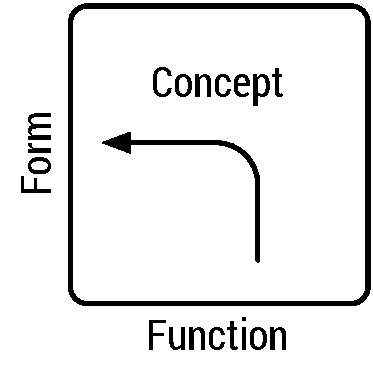
\includegraphics[width=\textwidth]{ffc.pdf}
		\end{column}
	\end{columns}

\end{frame}


\begin{frame}[fragile]
  \frametitle{Architecture is...}
  		\begin{center}
			\begin{quote}
			The embodiment of \textbf{concept}, and the allocation of physical/informational \textbf{function} to elements of \textbf{form}, and definition of \textbf{interfaces} among the elements and with the surrounding \textbf{context}.
			\end{quote}
		\end{center}
	\cite{edcrawley} 
\end{frame}

\begin{frame}[fragile]
  \frametitle{Definitsioonid}
	\begin{description}
		\item[Vorm] See, mis \emph{on} + selle miski struktuur
		\item[Funktsioon] See, mida tehakse struktureerituna peamist väärtust toova protsessi ümber
		\item[Kontseptsioon] Süsteemi visioon, mis seob vormi funktsiooniga ning kehastab peamisi printsiipe
	\end{description}
\end{frame}
\note{Kontseptsioon on see koht, kus mängu tuleb organisatsiooni kultuur, selle asjaga me veel kohtume! Just see vastab küsimusele, miks mõistlik lahendus samala probleemile on startupis ja pangas erinev}

\begin{frame}[fragile]
  \frametitle{Märkused mudeli kohta}
	\begin{itemize}
		\item Arhitektuur määrab disaini- ja operatiivparameetrid, disain annab neile väärtused
		\item Kuna mudel sisaldab nii funktsiooni kui vormi struktuuri, on mudel tihedalt seotud keerukuse kontseptsiooniga
		\item Väga multidistsiplinaarne lähenemine (inseneriteadus, juhtimine, kontrolliteooria, AI, matemaatika jne.)
		\item Olemuslikult holistiline ja seotud süsteemimõtlemisega 
	\end{itemize}
\end{frame}

%Arutelu koht
\begin{frame}[fragile]
  \frametitle{Arutelu koht}
		\begin{center}
			\textbf{Kui palju erineb toodud mudel harjumuspärasest?}
		\end{center}
\end{frame}

\section{Viited}

\begin{frame}[t,allowframebreaks,]
  	\bibliographystyle{plainnat}
	\bibliography{it_strateegia} 

\end{frame}

\section{Litsents}
\begin{frame}{Theme}

  Get the source of this theme and the demo presentation from

  \begin{center}\url{http://github.com/matze/mtheme}\end{center}

  The theme \emph{itself} is licensed under a
  \href{http://creativecommons.org/licenses/by-sa/4.0/}{Creative Commons
  Attribution-ShareAlike 4.0 International License}.

  \begin{center}\ccbysa\end{center}

\end{frame}

\begin{frame}{Sisu}
	The contents of the slides is lidecensed under a \href{http://creativecommons.org/licenses/by-nc-sa/4.0/}{Creative Commons Attribution-NonCommercial-ShareAlike 4.0 International}
	\begin{center}\ccbyncsa\end{center}
\end{frame}

\plain{Küsimusi?}

\end{document}